\documentclass[11pt]{article}
\usepackage{tocloft}
\usepackage{graphicx}
\usepackage{calc}
\usepackage{amssymb}
\usepackage{color}
\usepackage{array}
\usepackage[sc]{mathpazo}
\usepackage{url}
\usepackage[final]{pdfpages}
\usepackage{amsmath}

%\linespread{1.05}
\oddsidemargin=0pt
\evensidemargin=0pt
\textwidth=6.5in
\topmargin=0pt
\headheight=0pt
\headsep=0pt
\textheight=9in
% EXPERIMENTAL
%\parindent=0pt
%\parskip=3pt
\setlength{\parindent}{0cm}
\newcommand\secfont{\fontfamily{cmss}\selectfont}%\textwidth 5.5truein
\newcommand\pifheading[1]{{\secfont\textbf{#1}:}}
%\oddsidemargin -0.40truein
%\textheight 8.0truein
%\topmargin -0.25truein
\def\lo{
\mathrel{\raise.3ex\hbox{$<$}\mkern-14mu\lower0.6ex\hbox{$\sim$}}
}
\def\hi{
\mathrel{\raise.3ex\hbox{$>$}\mkern-14mu\lower0.6ex\hbox{$\sim$}}
}

\textwidth = 6.6 in
\textheight = 9.1 in
\oddsidemargin = -0.05 in
\evensidemargin = +0.05 in
\topmargin = -.1 in
\headheight = 0.0 in
\headsep = 0.0 in
\parskip = 0.06in
\newcommand\registered{{\ooalign{\hfil\raise .00ex\hbox{\scriptsize R}\hfil\crcr\mathhexbox20D}}}

%% Define a new 'leo' style for the package that will use a smaller font.
\makeatletter
\def\url@leostyle{%
  \@ifundefined{selectfont}{\def\UrlFont{\sf}}{\def\UrlFont{\small\ttfamily}}}
\makeatother
%% Now actually use the newly defined style.
\urlstyle{leostyle}

%\pagestyle{empty}
%\includeonly{previous,proposal_references}
%\includeonly{proposal_references}
%\includeonly{previous}

% TOC

\pagenumbering{gobble}

\begin{document}
%%%%%%%%%%%%%%%%%%%%%%%%%%%%%%%%%%%%%%%%%%%%%%%%%%%%%%%%%%%%%%%%%%%%%
\begin{center}
\textbf{\Large
AST101: Our Corner of the Universe \\
\vspace*{0.1cm}
Lab 7: Spectroscopy (I) DRAFT
}
\end{center}

\vspace*{0.5cm}

{\Large Name:}\vspace*{0.5cm}\\\hrule
{\Large Student number (SUID):}\vspace*{0.5cm}\\\hrule
{\Large Lab section:}\vspace*{0.5cm}\\\hrule
{\Large Group Members:}\vspace*{0.5cm}\\\hrule
\vspace*{0.5cm}

%%%%%%%%%%%%%%%%%%%%%%%%%%%%%%%%%%%%%%%%%%%%%%%%%%%%%%%%%%%%%%%%%%%%%

\section{Objectives}
\begin{itemize}
	\item To distinguish and describe the origins of both continuous spectra (usually thermal radiation) and line spectra (from atomic emission)
	\item To use a simulator to explore the basic properties of thermal radiation
\end{itemize}

\section{A note}
This lab involves several parts. Every group will need to spend some time experimenting with the long-wavelength cameras we have available to answer the last question. Some groups should work on the last question first, and then rotate back to the beginning of the lab.

\section{Introduction to Spectroscopy}

{\it Spectroscopy} is the practice of examining the different colors of light produced by something -- a {\it spectrum} -- to learn about
its properties.

For our purposes, there are two main types of spectra: continuous spectra (usually produced by a hot object as thermal radiation) and discrete spectra (usually produced by atomic transitions). For this week's lab, you will learn how to recognize and describe both of them, and then will study thermal radiation in a little more detail. Next week's lab is a detailed study in discrete spectra and atomic transitions.

\subsection{Thermal radiation and continuous spectra}

All objects emit light because of their temperature. This is called {\it thermal radiation}, and is always a broad, continuous spectrum of light. Thermal radiation doesn't just produce one or two specific wavelengths; it produces a continuous range of them. 

However, every thermal radiation spectrum will have one wavelength that is the brightest -- the wavelength where it emits more light than any other. We call this the {\it peak wavelength}.

The {\bf intensity of light} and {\bf peak wavelength of that light} depend on the object's temperature:

\begin{itemize}
\item Light from hotter objects has a {\it shorter} peak wavelength than light from colder objects. If you double the temperature of an object, the peak wavelength decreases by a factor of two.

\item Light from hotter objects is {\it overwhelmingly more intense} than light from colder objects. If you double the temperature of an object, the intensity of that light increases by a factor of sixteen.
\end{itemize}

You can determine the temperature of a hot object by looking at its peak wavelength. Objects with temperatures of thousands of Kelvin, like stars and fire, have a peak wavelength that is in (or near) the visible range; objects with temperatures of hundreds of Kelvin (like most things on Earth) have a peak wavelength that is deep into the infrared. What the object is made of doesn't matter very much -- only its temperature.

``Intensity'' here just means the amount of light per area produced by the surface of a hot object. We talk about intensity rather than total energy so we don't have to worry about the {\it size} of a glowing object. (Obviously, something larger will produce more total light!)

A few things other than thermal radiation can produce discrete spectra, too -- including LED lights. We won't worry about how they work, since there aren't any in space!

\subsection{Atomic transitions and discrete spectra}

Instead of producing a broad, continuous range of wavelengths, other light sources produce a {\it discrete spectrum}: they give off light
of only a few, specific frequencies. These light sources involve atoms transitioning from one energy level to the other. We will worry about the details of how this works next week; this week, it's enough to be able to recognize what these spectra look like.

\section{Recognizing and Measuring Spectra}

We have two different ways of examining spectra. One is by using a handheld device called a {\it spectroscope} to separate light into the individual wavelengths that make it up, and then looking at those. These are the plastic triangular things. They will physically show you 
the colors that are present in a light source. Continuous spectra look like a continuous band of color, like a rainbow; discrete spectra look like a few bright lines.

Your computers have digital spectrometers that produce a different sort of result. Instead of splitting the colors apart so your eyes can see them, they make a graph of intensity vs. wavelength, showing you how much light of each wavelength is present in a source.

To use the spectrometers, run ``Logger Pro'' on your computers. You will need to make one change in the settings. Choose ``Experiment'', then ``Change Units''. Select the one option that's available, and make sure that it is set to ``Intensity'' rather than ``Emission'' or ``Absorption''.

Then, you may click ``Collect'' (the play button at the top) to start and stop data collection. The graph will show you the wavelength on the horizontal axis (measured in nanometers) and the amount of light in that wavelength on the vertical axis. To rescale the vertical axis of the graph to account for changes in brightness, press Ctrl-J.

{\bf NOTE: Be careful with the cables connecting the computers to the probes. They are made of fiber-optic cable and are not cheap!}

The results that you get from the computer may have a little ``ripple'' in them, even if the source you're looking at emits the same amount of light at all frequencies. This is an imperfection in our instrument -- like all real scientific instruments, these aren't perfect!

\bigskip


\textbf{Question 1.} Some of the light sources in the room emit thermal radiation: they glow because they are hot. What do you expect their spectrum to look like through your handheld spectroscope?

\vspace{1.5cm}
(2) \hrulefill\\

\textbf{Question 2.} The light bulbs attached to the dimmer switches are this type of source. An incandescent light bulb is simply a wire that's heated with an electric current. Go look at one of them; describe in words what its spectrum looks like viewed through your spectroscope.

\vspace{1.5cm}
(2) \hrulefill\\


(2) \textbf{Question 3.} On the axes below, sketch what you expect the basic shape of the ``intensity vs. wavelength'' curve to look like. It doesn't matter if it's exactly right. Then look at it with the computer spectrometer, and compare what you see to your prediction.

\begin{center}
	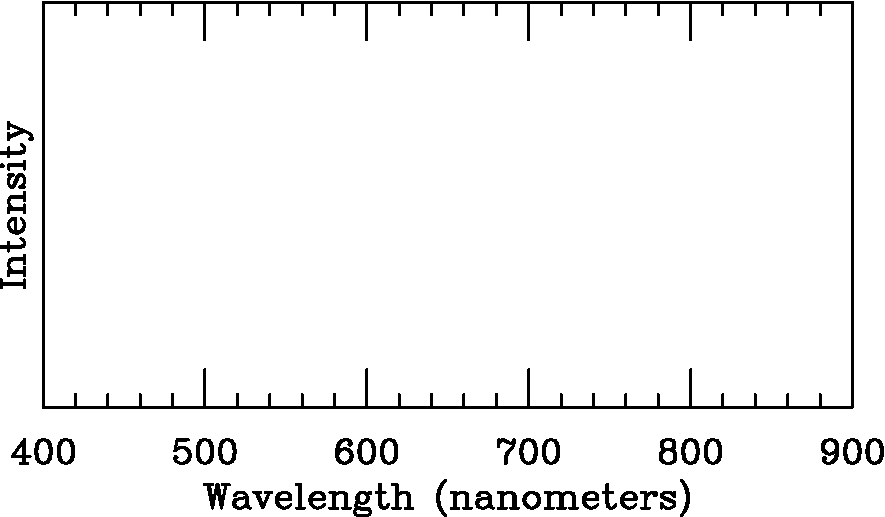
\includegraphics[width=0.6\textwidth]{spectrumplot-blank.pdf}
\end{center}
\newpage
(2) \textbf{Question 4.} Now, go to one of the computer stations next to the discharge tubes. Only turn these on when you're actively using them; they will overheat and burn out if you leave them on. Look at it first using the computer spectrometer. Draw what you see below:

\begin{center}
	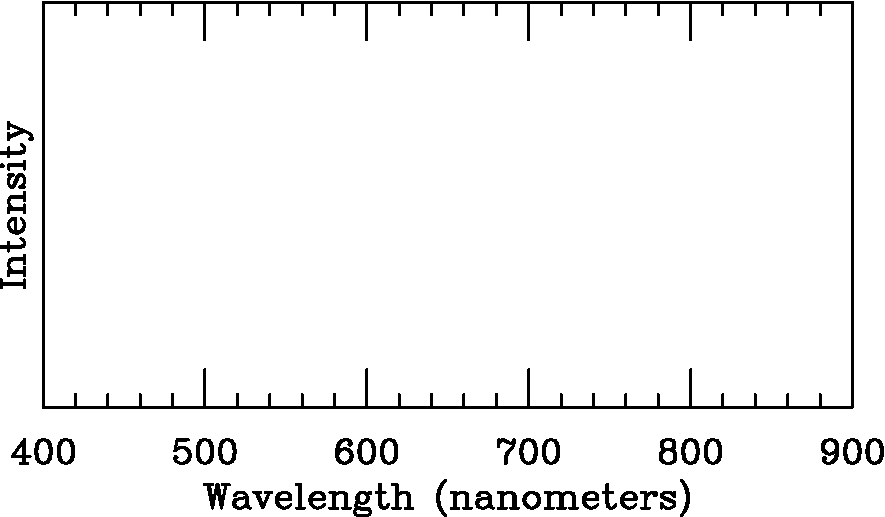
\includegraphics[width=0.6\textwidth]{spectrumplot-blank.pdf}
\end{center}

\textbf{Question 5.} Describe in words what you expect to see using your handheld spectroscope. Compare this to what you saw in Question 2, from the incandescent light bulb.

\vspace{1.5cm}
(2) \hrulefill\\


(4) \textbf{Question 6.} Now, go look at it using your handheld spectroscope. Draw what you see below. Notice that your spectroscope has markings for both energy per photon and wavelength in nm that you can use as landmarks; draw what you see as precisely as you can. (You
can indicate features by drawing with your pencil on top of the colors shown.) Note that depending on how you hold your spectroscope, the left-to-right axis on this picture may be reversed from what you see.

\begin{center}
	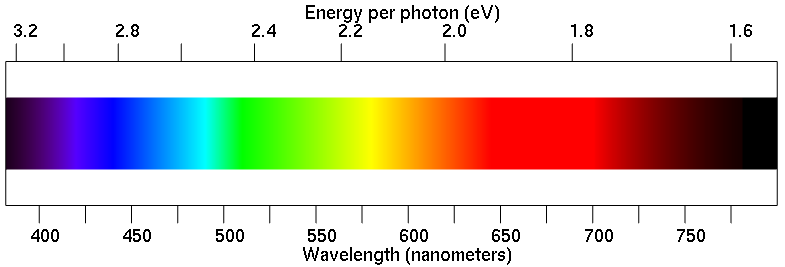
\includegraphics[width=0.8\textwidth]{spectrum2.png}
\end{center}
\newpage
\textbf{Question 7.} If it is daytime, point your spectroscope at something white or grey that's lit by the Sun: clouds, the sidewalk, a building, light coming from the window, etc. What do you see? Describe it in words. If it is dark outside, refer to the picture of 
the solar spectrum on the course website.


\vspace{1.5cm}
(2) \hrulefill\\

\textbf{Question 8.} Based on its spectrum, is the Sun likely to be emitting thermal radiation because it is hot, or emitting light for some other reason? Explain your answer.

\vspace{1.5cm}
(3) \hrulefill\\

\textbf{Question 9.} Are there any features of the Sun's spectrum that {\it don't} match your other experiences with spectra of this type? What is different about the Sun's spectrum from the light source in this room that most closely resembles it?

\vspace{2cm}
(4) \hrulefill\\

\textbf{Question 10.} Part of the power of spectroscopy is the ability to learn about something that produces light 
without actually accessing it. Use your spectroscope to look at the light coming from the ceiling in Holden Observatory.
Are they emitting thermal radiation like the incandescent light bulb, or do they work more like the discharge tubes? How do you know?

\vspace{2.5cm}
(4) \hrulefill\\

\textbf{Question 11.} Now, go into the Holden bathroom. You can't see the light bulbs directly since they're in those little frosted globes... but you can determine how they work with your spectroscope! What type of light bulb are they? How do you know?

\vspace{2cm}
(4) \hrulefill\\

\section{The Thermal Radiation (Blackbody) Simulator}

Go to the webpage \url {https://phet.colorado.edu/sims/html/blackbody-spectrum/latest/blackbody-spectrum_en.html} in Firefox, or some other browser that
supports Adobe Flash. This program generates thermal radiation (blackbody) curves given a temperature.

The horizontal axis indicates the wavelength of the emitted light and the vertical axis indicates the amount of energy per second (power) emitted by one square meter of the object at a particular wavelength.  

\subsection{The Sun's spectrum}

To start with, set the temperature to 5800 K.  Either move the slider or type the numbers in the temperature box. 5800 K is approximately the temperature of the Sun.  

Note that the horizontal axis specifies the emitted wavelengths $\lambda$ in units of micrometers, $\mu$m. One micrometer equals 1000 nanometers. (1$\mu$m = 1000 nm.)  For example, look at the visible spectrum.  The longest wavelength of the visible spectrum is approximately 0.7$\mu$m = 0.7x1000nm or 700nm.

{\bf Question 12.} Observe the peak of the curve.  The Sun emits the most energy at this wavelength.  We will label this wavelength $\lambda_{\rm peak}$ -- the wavelength where the curve is at its peak.

What color corresponds to $\lambda_{\rm peak}?$  What color is the Sun?


\vspace{2.5cm}
(2) \hrulefill\\



\textbf {Question 13.} What wavelength, numerically, is $\lambda_{\rm peak}$? Give your answer in both $\mu$m (the units used by this simulator), and nm (the units we usually use).

\vspace{2.5cm}
(2) \hrulefill\\
\newpage
\subsection{Other stars}

\textbf {Question 14.} Now, change the temperature to 7500 K, to simulate the thermal radiation from a hotter star. You'll again need to rescale the axes to make the graph fit on the screen.

In what two ways does this peak differ from that of the Sun?

\vspace{2cm}
(2) \hrulefill\\


\textbf {Question 15.} Suppose that you had a star with a temperature of 7500 K that was the same size as the Sun. How would its color and brightness differ from the Sun? Explain based on what you see in the simulator.

\vspace{2cm}
(2) \hrulefill\\

\textbf {Question 16.} The peak wavelength of a thermal radiation spectrum tells you the temperature of the object you're looking at; this is how astronomers can tell the temperature of stars. Go to one of the light bulbs connected to the dimmer switch. Using the digital spectrometer, determine the peak wavelength of its thermal radiation both at low power and at maximum power. Write these wavelengths down here:

\vspace{2cm}
(2) \hrulefill\\

\textbf {Question 17.} By comparing the simulated thermal radiation curves at different temperatures on your computer with your measurements from the previous question, determine the temperature of the light bulb's filament at low power and at maximum power. 

\vspace{3cm}
(5) \hrulefill\\

\newpage
\textbf {Question 18.} Betelgeuse is a red giant star that is only 3600 K. However, it's extremely bright -- around 100,000 times brighter than the Sun, when viewed from the same distance away. How could a cooler star be brighter than the Sun? Explain.

\vspace{2cm}
(3) \hrulefill\\

\textbf {Question 19.} Gradually reduce the temperature in the simulator. While you do, rescale the graph using both the ``zoom in/out'' controls to change the wavelength range, and the ``+ / -'' controls you used before to change the intensity range. Go down to 300 K --
the temperature of things around us. What range of wavelengths do they mostly emit? (Give your answer in both $\mu$m and nm.) How does this compare to the visible-light spectrum? 

\vspace{3cm}
(3) \hrulefill\\

\newpage

(8) \textbf {Question 20.} We have special cameras that can see much longer wavelengths than our eyes can for you to use. Point one of them at different objects around the room: people, hot and cold drink containers, clothing of different colors, electronics that are running, and the like. Rather than asking you to do something specific, I'd like you to make some interesting observations on your own. Address questions like: How do you think the special camera works? What is the relation between the color of the object and how it shows up on the camera? How does the camera interact with visible light produced by the lights in the room? If it doesn't see light reflected from the lights in the room, does it detect light at all? Where does that light come from?

If you'd like to take pictures of yourself or friends with these, you can do that! You can download those pictures from the cameras by using USB cables to attach them to your computer or the computers in the room; if you use the computers in the room, you'll need to send them to yourself somehow.


\end{document}